%% Copyright (c) 2015-2019, RTE (http://www.rte-france.com)
%% See AUTHORS.txt
%% All rights reserved.
%% This Source Code Form is subject to the terms of the Mozilla Public
%% License, v. 2.0. If a copy of the MPL was not distributed with this
%% file, You can obtain one at http://mozilla.org/MPL/2.0/.
%% SPDX-License-Identifier: MPL-2.0

%% This file is part of Dynawo, an hybrid C++/Modelica open source time domain
%% simulation tool for power systems.

\documentclass[a4paper, 12pt]{report}
\usepackage{graphicx}
\usepackage{float}
\usepackage{listings}
\usepackage{tikz}
\usepackage{array}
\usepackage{pgfplots} %for graphics
\usepackage{schemabloc}
\pgfplotsset{compat=newest}
\usetikzlibrary[pgfplots.groupplots]
\usepgfplotslibrary{groupplots}
\usetikzlibrary{shapes,matrix,arrows,decorations.pathmorphing}
\definecolor{myblue}{rgb}{0.0,0.57,0.81}
\definecolor{myred}{rgb}{0.86,0,0.17}
\definecolor{mygreen}{rgb}{0,0.58,0}
\definecolor{mygray}{rgb}{0.4,0.4,0.4}
\definecolor{myyellow}{rgb}{1,0.84,0.024}
\definecolor{mycyan}{rgb}{0.19,0.835,0.87}
\definecolor{mypurple}{rgb}{0.635,0.055,0.67}
\definecolor{myorange}{rgb}{0.86,0.44,0.145}
\definecolor{myblueT}{rgb}{0.082,0.48,0.76}
\definecolor{myredT}{rgb}{0.84,0.18,0.18}



\begin{document}

\chapter*{Test - "Governor Proportional"}
This is the documentation for the test "GovernorProportional" in the Dyna$\omega$o project non regression tests.

% Generic description of the non regression test
% Data origin, network size, simulation types and numbers, etc.
\section*{Test description}

This document presents a basic unit test based on a DYD file which instantiates Proportional Governor model whose target pulsation and control pulsation are connected to step models.


\tikzstyle{block} = [draw, fill=blue!20, rectangle,
    minimum height=3em, minimum width=6em]
\tikzstyle{sum} = [draw, fill=blue!20, circle, node distance=1cm]
\tikzstyle{input} = [coordinate]
\tikzstyle{output} = [coordinate]
\tikzstyle{pinstyle} = [pin edge={to-,thin,black}]

\begin{figure}[H]
  \setlength{\belowcaptionskip}{15pt}
  \caption{Block diagram of a Proportional Governor coupled to a synchronous machine}
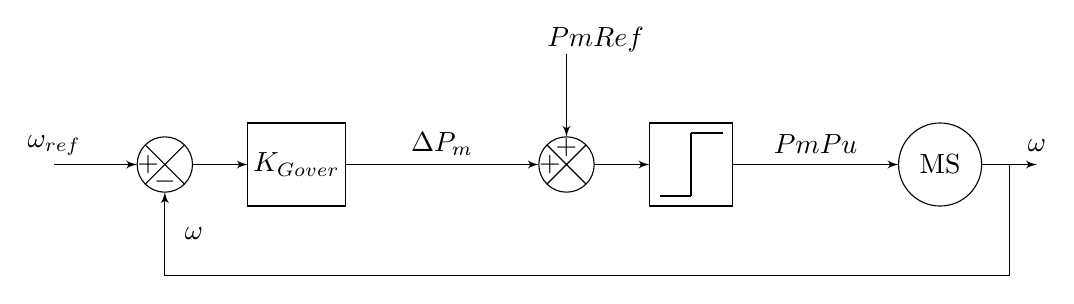
\begin{tikzpicture}[every node/.style={inner sep=0,outer sep=0}]
\sbEntree{E}
\sbComp{a}{E}
\sbStyleLien{node distance=1em}
\sbRelier[]{E}{a}
\sbNomLien[0.7]{E}{$\omega_{ref}$}
\sbStyleBloc{inner xsep=2}
\sbBlocL{b}{$K_{Gover}$}{a}
\sbStyleBlocDefaut
\sbSumh[8]{c}{b}
\sbRelier[]{b}{c}
\sbNomLien[0.7]{b-c}{$\Delta P_m$}
\sbDecaleNoeudy[-4]{c}{Py}
\sbRelier[]{Py}{c}{}
\sbDecaleNoeudx[1]{Py-c}{DPm}
\sbNomLien[2]{DPm}{$PmRef$}
\sbBlocL{d}{\tikz {\draw (-0.4,-0.4) -- (0,-0.4);\draw (0,-0.4) -- (0,0.4); \draw (0,0.4) -- (0.4,0.4); }}{c}
\sbStyleBloc{circle}
\sbBlocL[6]{e}{MS}{d}
\sbNomLien[0.7]{d-e}{$PmPu$}
\sbStyleBlocDefaut
\sbSortie{S}{e}
\sbRelier{e}{S}
\sbNomLien[0.7]{S}{$\omega$}
\sbRenvoi{e-S}{a}{}
\sbDecaleNoeudx[1]{e-S-a}{ret}
\sbNomLien[0]{ret}{$\omega$}
\end{tikzpicture}
\end{figure}


% Description of the simulation
% Events, solver, duration, outputs, etc.
\subsection*{Simulation description}

Here are the important settings:

Gover parameters:
\begin{itemize}
\item The initial state is: target pulsation $\omega RefPu$=1, control pulsation $\omega Pu_0$=1, $PmPu_0$=1 .
\item The proportional $K_{Gover}$=1.
\item Power bounds: $PMin$=0.7 and $PMax$=1.3
\item $PNom$=1
\item We use the Simplified Solver.
\end{itemize}

Simulation development
\begin{itemize}
\item At $t=0s$, $\omega Pu$=1;
\item At $t=40s$, $\omega Pu$=0.6;
\item The simulation lasts for 80s.
\end{itemize}


% Expected results
% Events, logs, plots, etc.
\subsection*{Expected results}
\subsubsection*{Governor Proportional test}

In this test, we expect:


\begin{itemize}
\item At $t=0s$, $\omega RefPu$ - $\omega Pu$ = 0 so $PmPu$ = $PmPu_0$ = 1.
\item At $t=40s$, $\omega RefPu$ - $\omega Pu$ = 0.4 so $PmRawPu$ = 1.4. We expect the Governor to detect that the upper bound $PMaxPu$ is reached and $PmPu$=1.3 .
\end{itemize}

The following plots illustrate the aforementioned points:


\begin{figure}[H]
  \caption{Proportional Governor output PmPu (p.u)}
  \begin{tikzpicture}
    \begin{axis}[
        axis background/.style={fill=white},
        %title = {\begin{small}Evolution of Governor output EfdPu as a function of time (p.u)\end{small}},
        ymin = 0.9,
        ymax = 1.7,
        xmin = 0,
        xmax = 80,
        xtick= {0,10,...,80},
        ytick= {0.5,0.7,...,1.5},
        x label style={at={(axis description cs:0.5,-0.15)},anchor=north},
        y label style={at={(axis description cs:0.,0.45)},anchor=south},
        xlabel={\begin{small}$time$ (s)\end{small}},
        height=0.6\textwidth,
        width=1\textwidth
        ]
        \addplot[color=myred!50,no markers,line width=1pt,each nth point={1}]
        table[x=time,y=GoverProp_Gover_PmPu, col sep=semicolon]
        {../reference/outputs/curves/GoverProportional.csv};
        \addplot[color=myblue!50,no markers,line width=1pt,each nth point={1}]
        table[x=time,y=GoverProp_Gover_PmRawPu_y, col sep=semicolon]
        {../reference/outputs/curves/GoverProportional.csv};
        \legend{$PmPu$, $PmRawPu$}
    \end{axis}
  \end{tikzpicture}
\end{figure}

\begin{figure}[H]
  \caption{Proportional Gover inputs $\omega RefPu$ and $\omega Pu$ (p.u)}
  \begin{tikzpicture}
    \begin{axis}[
        axis background/.style={fill=white},
        %title = {\begin{small}Evolution of Gover inputs UcEfdPu and UsPu as a function of time (p.u)\end{small}},
        ymin = 0.5,
        ymax = 1.5,
        xmin = 0,
        xmax = 80,
        xtick= {0,10,...,80},
        ytick= {0.5,0.7,...,1.5},
        x label style={at={(axis description cs:0.5,-0.15)},anchor=north},
        y label style={at={(axis description cs:0.,0.45)},anchor=south},
        xlabel={\begin{small}$time$ (s)\end{small}},
        height=0.6\textwidth,
        width=1\textwidth
        ]
        \addplot[color=myred!50,no markers,line width=1pt,each nth point={1}]
        table[x=time,y=GoverProp_Gover_omegaPu, col sep=semicolon]
        {../reference/outputs/curves/GoverProportional.csv};
        \addplot[color=myblue!50,no markers,line width=1pt,each nth point={1}]
        table[x=time,y=GoverProp_Gover_omegaRefPu_y, col sep=semicolon]
        {../reference/outputs/curves/GoverProportional.csv};
        \legend{$\omega Pu$, $\omega RefPu$}
    \end{axis}
  \end{tikzpicture}
\end{figure}

This correspond to the following timeline :
\lstinputlisting[breaklines, frame = lines, framesep = 2em]{../reference/outputs/timeLine/timeline.log}




\end{document}
